\documentclass{article}
\usepackage[utf8]{inputenc}

%\usepackage[english]{babel}
%\usepackage[utf8x]{inputenc}
\usepackage{fullpage}
\usepackage{subcaption} %Subfigure
%\usepackage{subfigure} %Subfigure
\usepackage{pifont}
\usepackage{latexsym}
\usepackage{mathrsfs}
\usepackage{amssymb,amsbsy}
\usepackage{amsmath}     
\usepackage{amsfonts}
\usepackage{graphicx}
\usepackage{tcolorbox}
\usepackage[colorinlistoftodos]{todonotes}
\usepackage{varwidth}
%\usepackage{authblk}
\usepackage{algorithm}
\usepackage[ruled,vlined]{algorithm2e}
\usepackage{algorithmic}
\usepackage{lmodern}
\usepackage{natbib}
\usepackage{mathtools}      
\usepackage[titletoc]{appendix}
%\usepackage{titlesec}       
\usepackage{titletoc}
\usepackage{ntheorem}
\DeclareMathOperator{\Hessian}{Hess}

%\graphicspath{{Images/}}
\usepackage{graphicx}
\usepackage{epsfig}
%% The amssymb package provides various useful mathematical symbols
\usepackage{amssymb}
\usepackage{amsmath}  
\usepackage{float}
\newfloat{algorithm}{t}{lop}
\usepackage{lipsum}% http://ctan.org/pkg/lipsum
\usepackage{tikz}   %allows shapes of nodes
\usetikzlibrary{shapes,arrows}
%\usetikzlibrary{positioning,chains,fit,shapes,calc}
%\usetikzlibrary{trees} 
%\usepackage{tkz-graph}
\usetikzlibrary{positioning, automata}
\usepackage{makeidx}         % allows index generation
 \usepackage{blkarray}% http://ctan.org/pkg/blkarray
 \newcommand{\matindex}[1]{\mbox{\scriptsize#1}}% Matrix index
 \usepackage{dcolumn}
\newcolumntype{L}{D{.}{.}{1.1}}
\usepackage{multirow}% http://ctan.org/pkg/multirow
\usepackage{hhline}% http://ctan.org/pkg/hhline
\usepackage{caption}
%\captionsetup{labelsep=space,justification=justified,singlelinecheck=off}
 \usepackage{fancyhdr,graphicx,amsmath,amssymb}
%\usepackage[ruled,vlined]{algorithm2e}

%%%%%%%%%%%%%%%%%%%%%%%%%%%%
% Code Listing for Python code
\definecolor{codegreen}{rgb}{0,0.6,0}
\definecolor{codegray}{rgb}{0.5,0.5,0.5}
\definecolor{codepurple}{rgb}{0.58,0,0.82}
\definecolor{backcolour}{rgb}{0.95,0.95,0.92}

\usepackage{listings}
\include{pythonlisting}
\lstdefinestyle{mystyle}{
  backgroundcolor=\color{backcolour},   commentstyle=\color{codegreen},
  keywordstyle=\color{magenta},
  numberstyle=\tiny\color{codegray},
  stringstyle=\color{codepurple},
  basicstyle=\ttfamily\footnotesize,
  breakatwhitespace=false,         
  breaklines=true,                 
  captionpos=b,                    
  keepspaces=true,                 
  numbers=left,                    
  numbersep=5pt,                  
  showspaces=false,                
  showstringspaces=false,
  showtabs=false,                  
  tabsize=2
}

%"mystyle" code listing set
\lstset{style=mystyle}
 
\usepackage[bottom]{footmisc}% places footnotes at page bottom
\usepackage{algorithm, algpseudocode} 
\captionsetup{compatibility=false} 
\usepackage{listings}
\floatstyle{plain} % Box...
%\restylefloat{figure}% ...figure environment contents.






%for JSON
\usepackage{bera}% optional: just to have a nice mono-spaced font
\usepackage{listings}
\usepackage{xcolor}
\title{Discrete Structures of Computer Science\\
Project--Faculty Assignment}
\author{Aditya Chaudhary(2022A7PS0622G)\\
         Pray Raskapoorwala(2022A7PS1239G)\\
         Aditya  Gupta(2022A7PS0090G)}
\date{28 November 2023}

\begin{document}

\maketitle
%Derivations
\section{Problem Statement}
The problem at hand involves the faculty allocation problem,which aims to allocate courses to faculty based on their preferences and workload while also making sure that all the courses have been alloted and \textbf{no course remains empty,if the course is a Compoulsary Disciplinary Elective(CDC),while it may or may not be alloted if it is an elective}
Through the allocation,we need to make sure that maximum courses are alloted according to the preferences of the professor.
Some of the given constraints are:\begin{itemize}
    \item The professors are divided into three categories-The first category can take 0.5(half) of a course,the second category professors can take 1(full) course and the third category can take 1.5 courses(i.e. either half,full or 1.5).
    \item There is no prioritization between professors in the same category
\end{itemize}

\section{Assumptions}
\begin{itemize}
 

\item The preferences of the professors are multiplied by 2 since we cannot compare two \textbf{floating point numbers} for equality.

\hspace{1cm}

 \item We are assuming that all CDC's are alloted,and the sum of all the workloads of the professors should be equal to the total number of courses available,i.e.\\

  \hspace{1cm}
  \sum_{i} \mathbf{Workload}(i) = \mathbf{Total\ number\ of\ courses}
  

\end{itemize}

\hspace{2cm}

\section{Approach}:\begin{itemize}
The approach we used was\textbf{ linear programming and making constraints from Matrix Manipulation}. The steps include:\\
\item We have given two codes for CDCs and Electives as there is a slight change in their constraints.\\
 \item We assumed there are n professors and each professor gives preference for n courses involves some CDC's and electives\\
\item To begin with a smaller testcase,we assumed a matrix of order 4 wherein the preferences for the courses were listed in the corresponding rows,i.e. \\
    \hspace{2cm}



   
     \matrixTitle  Preference Matrix=
    \begin{bmatrix}
   Prof/Course& Course A&Course B&Course C&Course D\\
      Prof1&    1 & 1 & 0 & 0 \\
   Prof2& 0 & 2 & 2 & 0 \\
    Prof3&3 & 0 & 0 & 3 \\
    Prof4&0 & 2 & 2 & 0 \\
    \end{bmatrix}
    


\hspace{1cm}


 
  \begin{itemize}
    \item The courses are represented by $A$, $B$, $C$, and $D$, and the preferences are given by:
    \begin{itemize}
        \item $1$ if a professor of the first category has given preference for the course.
        \item $2$ if a professor of the second category has given preference for the course.
        \item $3$ if a professor of the third category has given preference for the course.
        \item $0$ if a professor does not give preference for the course.
    \end{itemize}
\end{itemize}

  \hspace{1cm}

 \item Then we multiplied the above matrix with:

\[
  \matrixTitle Variable Matrix=
    \begin{bmatrix}
w1 & w2 & w3 & w4 \\
x1 & x2 & x3 & x4 \\
y1 & y2 & y3 & y4 \\
z1 & z2 & z3 & z4 \\

\end{bmatrix}


\]
\item For the above matrix,we introduced some dummy variables, which are:(\textbf{Note: All the variables will only take integer value for solution)}
    \begin{itemize}
        \item $W_i$ for faculty $i$ giving preference to course A,
        \item $X_i$ for faculty $i$ giving preference to course B,
        \item $Y_i$ for faculty $i$ giving preference to course C,
        \item $Z_i$ for faculty $i$ giving preference to course D.
    \end{itemize}

Subject to the constraint: $\sum_{j=1}^{4} A_{i,j} = 2$ for each row $i$.

\item The obtained product is \begin{bmatrix}
w1&w2 & w3 & w4 \\
x1 & x2 & x3 & x4 \\
y1 & y2 & y3 & y4 \\
z1 & z2 & z3 & z4 \\

\end{bmatrix}




  \item Then,we formulated some linear equations to satisfy the given constraints and provided a solution.

  \item The equations are:
  \item $w1 + w2 = 1$
  \item $x2 + x3 =2$
  \item $z2 + z3 =2$
  \item $y1 + y4 =3$
  \item $w1 + y1 =2$
  \item $w2 + x2+z2 =2$
  \item $y4 =2$
  \item $x3+z3 =2$

  \item These equations can be solved using Linear Algebra; there are multiple libraries in Python to solve linear Algebra Equations using different Constraints (Eg-Pulp). For this project, we are using Google OR-Tools library:
  To Install Google Or-Tools:\\\\
   \hspace{1cm}
    \textbf{python3 -m pip install -U --user ortools}
\\

  
\item Then, inputs for the number of courses and the professors' preferences were taken as run-time user input. The input is given at runtime, but we have introduced a jpg representing the user input taken for the particular case to read that input easily. Correspondingly, the output.txt file was made to assign the courses to the professors and to find the number of solutions(if the optimal solution is possible).

\item We then modeled this logic using some libraries in the ORTools to get all combinations and also to find if the solution is optimal or not


\end{itemize}







%Derivations
\section{Crash Test}

\begin{itemize}
    \item The crash test refers to a test case where the code would not work optimally.
\item Here, the crash test would be a case where all the courses have not been allotted to a professor or a case where the total number of courses taken by a professor exceeds his course limit.
\item Also, the code takes some time to run if the number of CDCs/Electives is more than 10.
\item Another aspect where the code might not work would be invalid inputs,i.e., the user might enter invalid inputs(e.g., a string instead of an integer in the course load of the professor). Now, we examine some cases:

\subsection{Crash Test 1}

\begin{figure }
  \subcaptionbox*{Input matrix}[0.8\linewidth]{%
    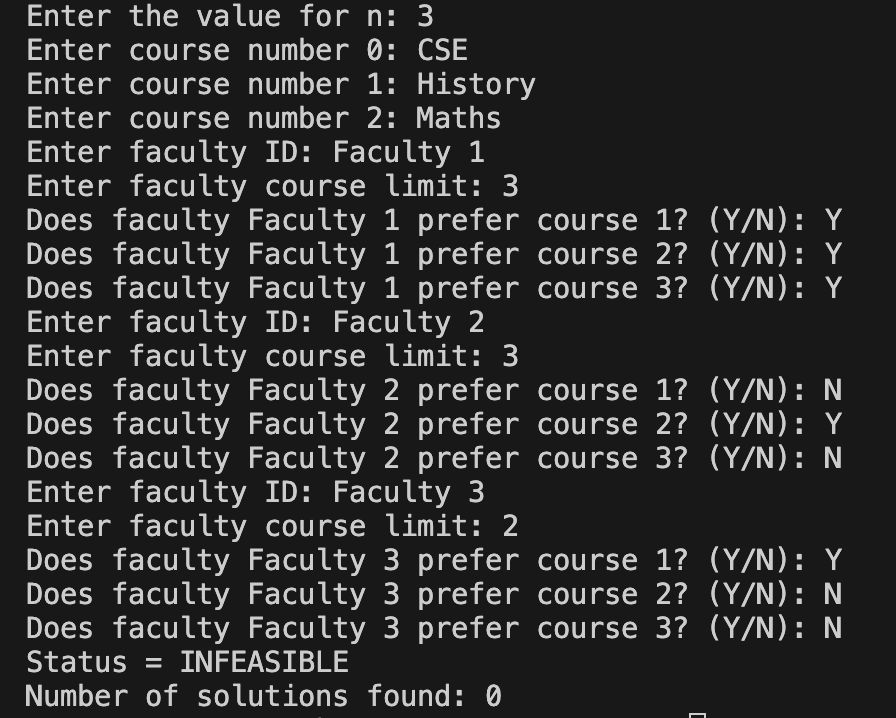
\includegraphics[width=\linewidth]{WhatsApp Image 2023-11-29 at 02.53.03.jpeg}
  }%
  \item As we can see the status of our solution is INFEASIBLE and we cannot get any possible combinations.This is because the \textbf{workload has exceeded the total number of courses(which contradicts our assumption and hence infeasible)}
  
\end{figure}

\subsection{Crash Test 2}

\begin{figure }
  \subcaptionbox*{Input matrix}[\linewidth]{%
    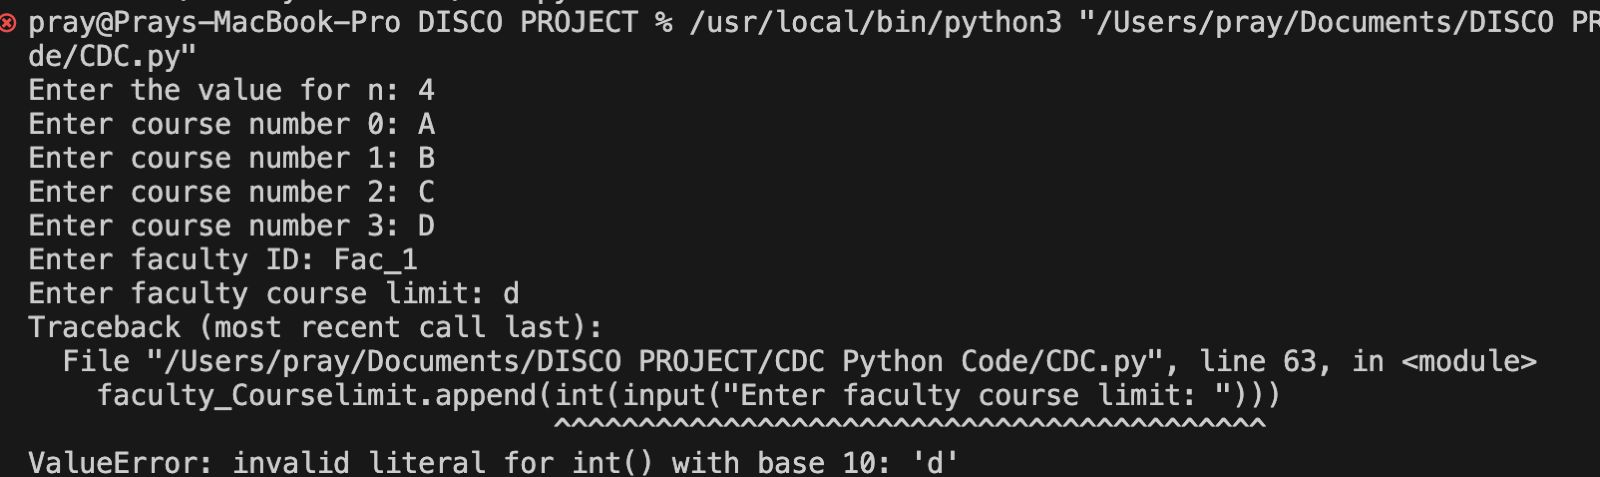
\includegraphics[width=\linewidth]{Invalid input.jpeg}
    
  }%
  \item Here,we can see that the input added is a string instead of an integer,so we are getting an error
  
\end{figure}

\end{itemize}

%Derivations
\section{Consistency Report}
\subsection{Testing for CDC's}
\subsubsection{Case 1}
For the given  testcase:
\begin{itemize}
    \item 

\begin{bmatrix}
   Professor/Course&CS F214-LCS&CS F222-DISCO&CS F215-DD&CS F213-OOP\\
   Professor 1&1 & 1& 0 & 0 \\
 Professor 2&0 & 2 & 2 & 0 \\
 Professor 3&3& 0 & 0 & 3 \\
 Professor 4&0 & 2 & 2 & 0  \\
\end{bmatrix}
we got \textbf{3 optimal solutions},which is consistent with the answer we got while physically iterating and generating the outputs.Those solutions are\\
\begin{figure}[ht]
  \subcaptionbox*{Status of the output}[.45\linewidth]{%
    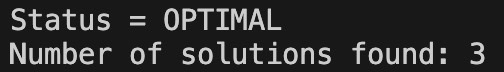
\includegraphics[width=\linewidth]{99F5BC90-F147-498B-8215-74588D257459_4_5005_c.jpeg}%
  }%
  \hfill
  \subcaptionbox*{All possible combinations}[.45\linewidth]{%
    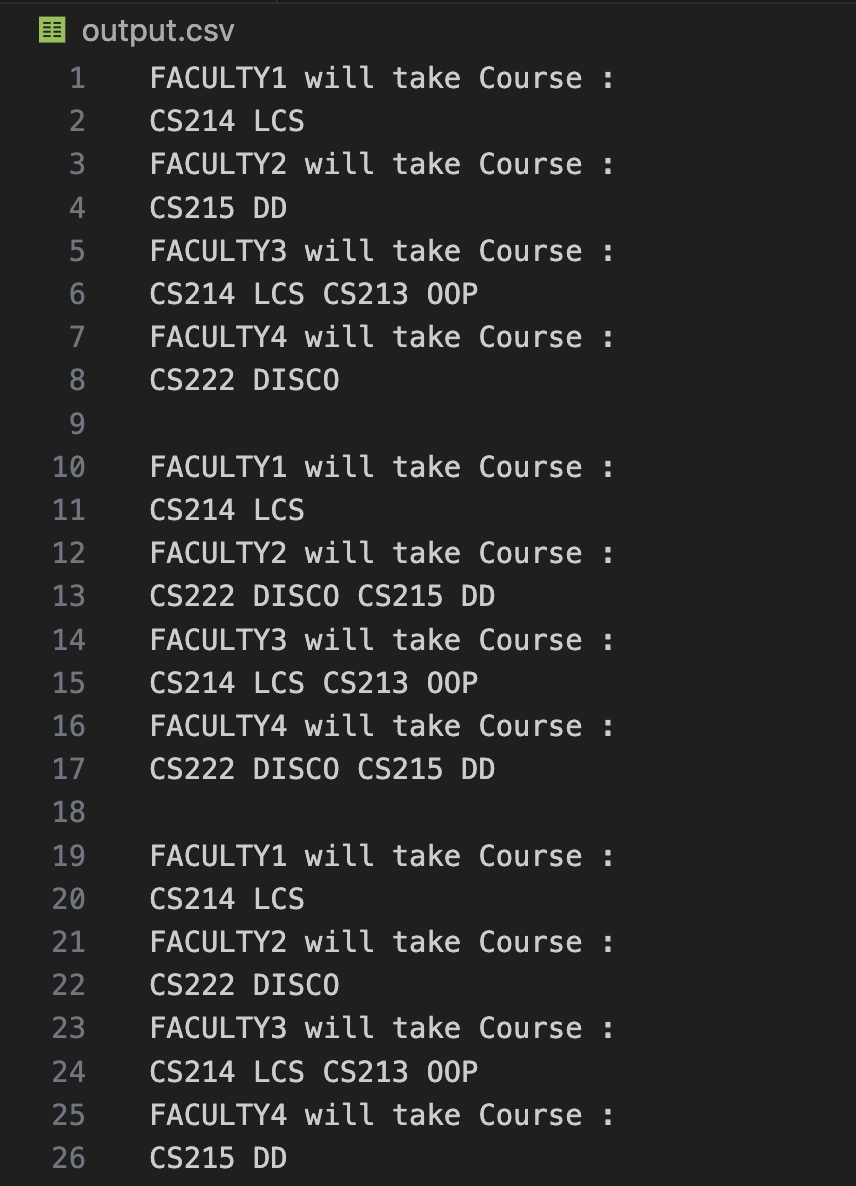
\includegraphics[width=\linewidth]{38AD138C-6CB2-488C-9CF1-1AA7870D3892.jpeg}%
  }
  \caption{Case of 4 CDC's}
\end{figure}


\subsubsection{Case 2}We now try to take a more complex example where the number of professors and courses are  8 and try to find the solution:
\begin{figure}[ht]
  \subcaptionbox*{Input matrix}[\linewidth]{%
    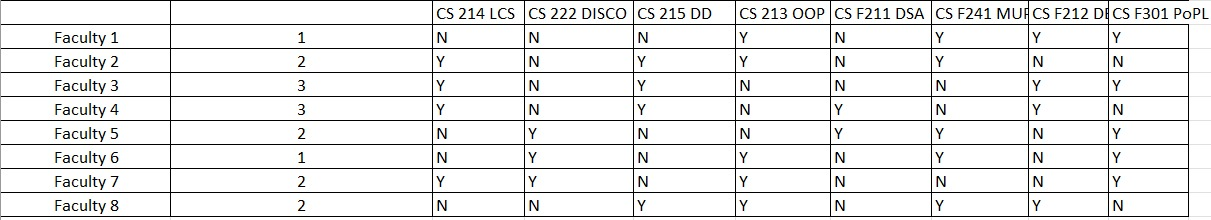
\includegraphics[width=\linewidth]{WhatsApp Image 2023-11-29 at 01.36.52.jpeg}
  }%
  
\end{figure}

\begin{figure }
  \subcaptionbox*{Status of the output}[.45\linewidth]{%
    
\includegraphics[width=\linewidth]{WhatsApp Image 2023-11-29 at 01.44.12.jpeg}%
  }%
  \hfill
  \subcaptionbox*{One of the  possible combinations}[.45\linewidth]{%
    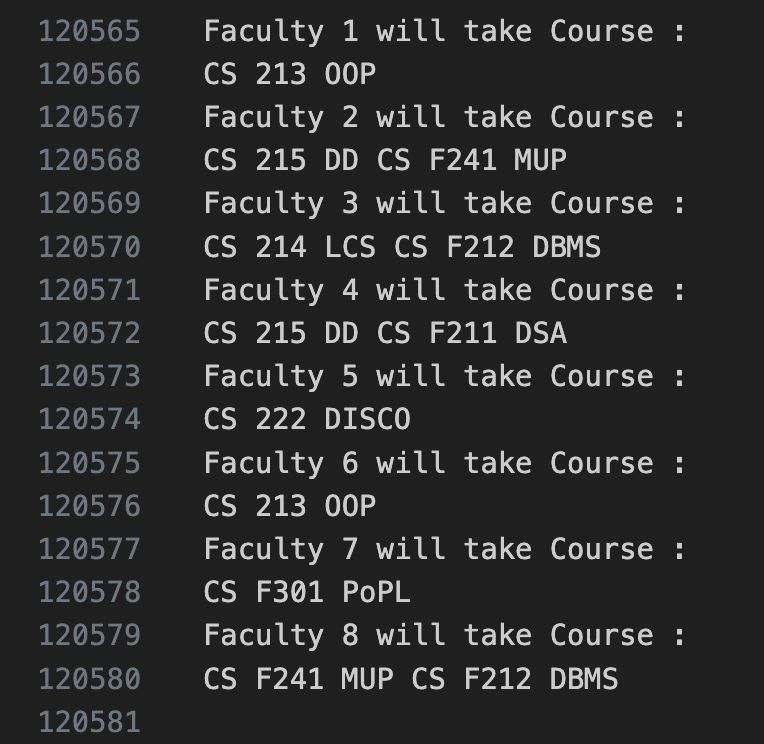
\includegraphics[width=\linewidth]{WhatsApp Image 2023-11-29 at 01.44.53.jpeg}%
  }
  \caption{Case of 8 CDC's}
\end{figure}

 \hspace{2 cm}

 Hence,we see that as the number of professors increases the total possible course assignments also increase.
 
\subsection{Testing for electives}-\textbf{The constraint to be kept in mind is that a few electives may not be assigned to any of the professors.}


\subsubsection{Case 1}Considering 2 electives:

\begin{bmatrix}
   Professor/Course&BITS F312-Neural Networks and Fuzzy Logic&BITS F343-Fuzzy Logic and Applications\\
   Professor 1&2&0 \\
Professor 2&0&3  \\
\end{bmatrix}

The output obtained is:
\begin{figure }
  \subcaptionbox*{Status of the output }[.45\linewidth]{%
    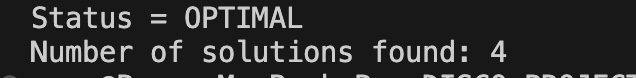
\includegraphics[scale=0.25]{Image 29-11-23 at 00.23.jpg}%
  }%
  \hfill
  \subcaptionbox*{All possible combinations}[.45\linewidth]{%
    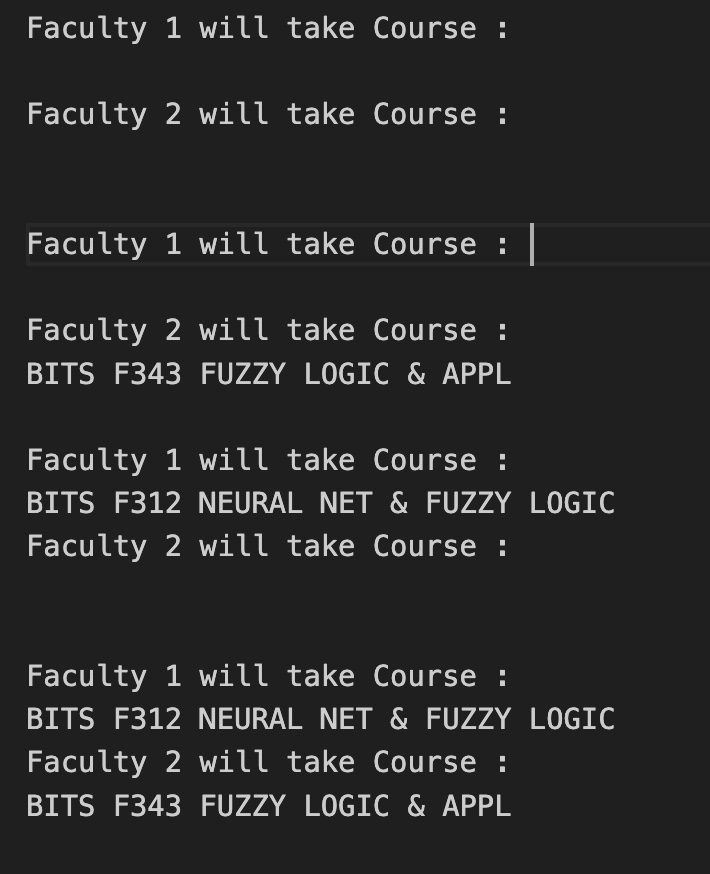
\includegraphics[scale=0.25]{Image 29-11-23 at 00.24.jpg}%
  }
  \caption{Case of 2 electives}
\end{figure}


\subsubsection{Case 2}
Here, we introduce another example of 5 electives.
\begin{figure}[ht]
  \subcaptionbox*{Input matrix}[\linewidth]{%
    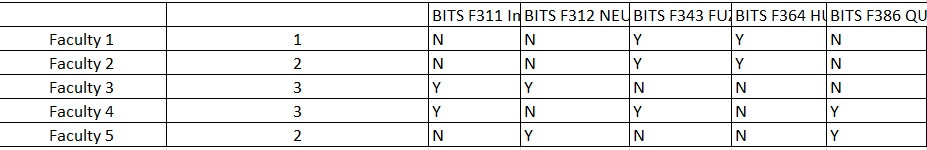
\includegraphics[width=\linewidth]{WhatsApp Image 2023-11-29 at 01.08.45.jpeg}
  }%
  
\end{figure}

\begin{figure }
  \centering
  \begin{minipage}[b]{\textwidth}
    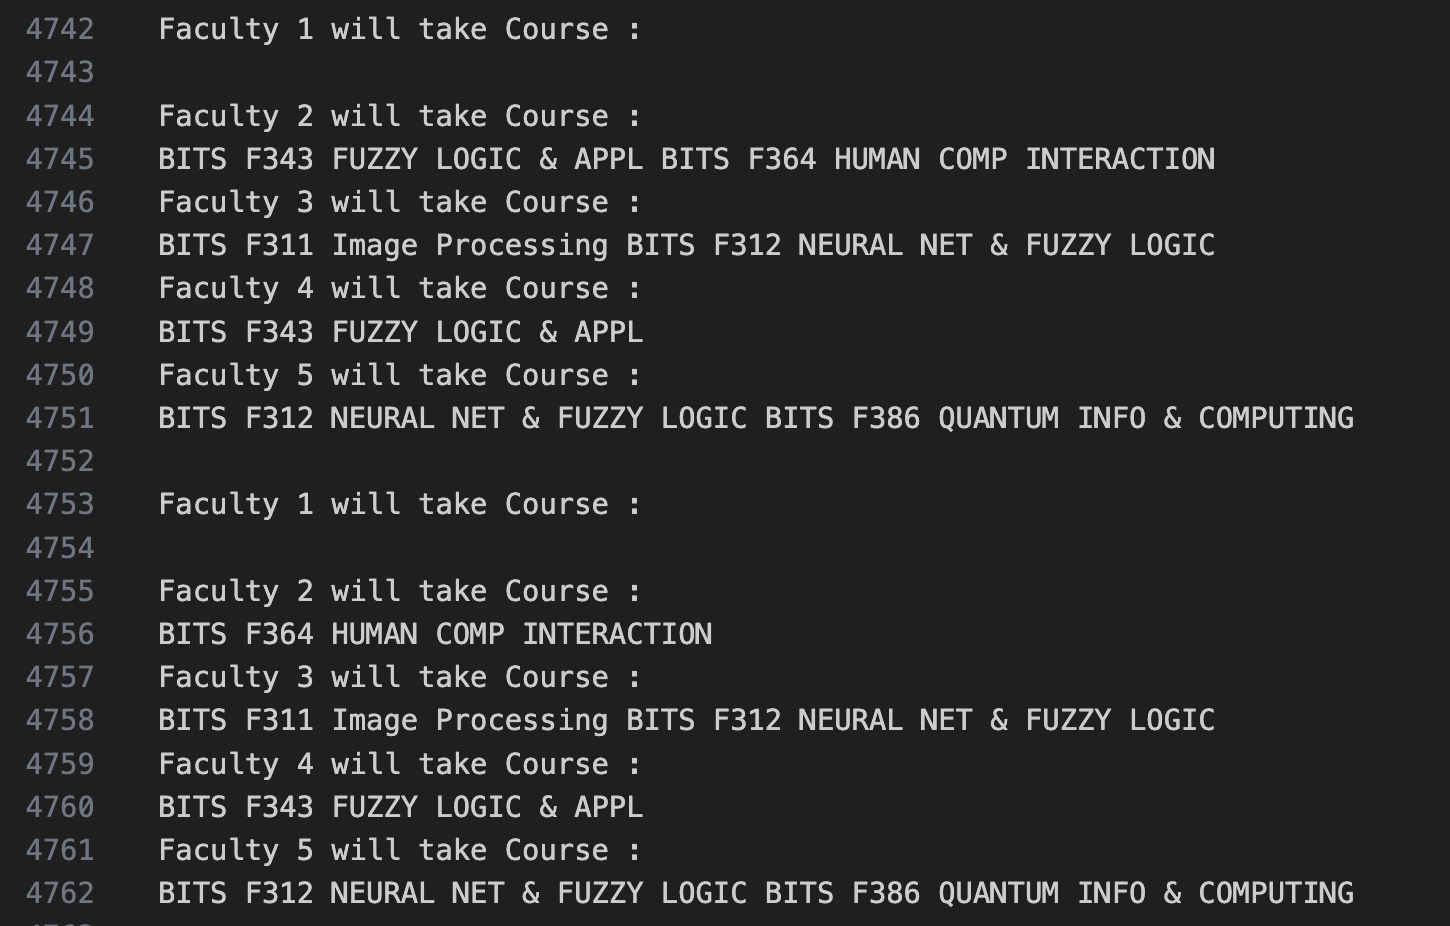
\includegraphics[width=\textwidth]{WhatsApp Image 2023-11-29 at 01.33.57.jpeg}
    \caption{One of the possible combinations}
  \end{minipage}
  \hfill
  \begin{minipage}[b]{0.4\textwidth}
    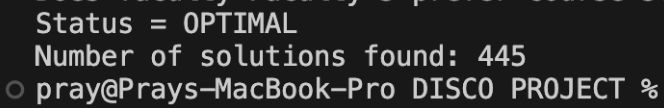
\includegraphics[width=\textwidth]{WhatsApp Image 2023-11-29 at 01.38.47.jpeg}
    \caption{Status of the solution}
  \end{minipage}
\end{figure}






\end{itemize}
\section{Conclusion}Hence,we see that the code is consistent for a variety of testcases for both CDC's as well as Electives.
We would like to thank Prof. Snehanshu Saha for this opportunity to do this project which made  us understand many new things and improved our problem solving skills 
\end{document}
https://www.overleaf.com/project/656304b2567ee1e3cf0380b1